\chapter{Materiales Semiconductores}

\section{Introducción}

Los materiales se clasifican en: conductores, semiconductores y aislantes. El parámetro que determina tal clasificación es la conductividad, que indica el grado o facilidad con la que permiten el paso de un flujo de portadores bajo un campo eléctrico externo. La inversa de la conductividad es la resistividad, propiedad intrínseca de los materiales.

En los semiconductores se puede modificar su resistividad de manera controlada entre márgenes muy amplios. Depende de la estructura atómica y del enlace atómico. El germanio y el silicio, son dos de los materiales semiconductores más importantes, que poseen cuatro electrones de valencia en su última capa.

\section{Obtención de cristales semiconductores}

Se parte de silicio monocristalino de grado semiconductor. Tiene una pureza de $10 ppb$. La materia prima de partida es el sílice (SiO2). Se purifica la materia prima mediante procesos físicos y químicos.

\textbf{Proceso químico}

\begin{enumerate}
    \item Obtención de la materia prima (SiO2)
    \item Eliminación del oxígeno del SiO2, por reducción por carbono
    \item Cloración
    \item Destilación fraccionada
    \item Reducción del triclorosilano (SiHCl3) para obtener el Si
\end{enumerate} 

\textbf{Proceso físico}
\begin{enumerate}
    \item Purificación por refinado de zona basado en el mayor coeficiente dee solubilidad de las impurezas en el material en estado líquido que en estado sólido
    \item El cristal se coloca en posición vertical y se va calentando en horno por radiofrecuencia
\end{enumerate}

\section{Crecimiento de monocristales - Método Czochralski}

Consiste en la obtención de un lingote de Si monocristalino a partir de material líquido contenido en un crisol.

\begin{enumerate}
    \item En un crisol, se funde Si grado semiconductor a 1400ºC.
    \item Se pone en contacto con la superficie líquida, una ``semilla''del mismo material monocristalino.
    \item Se hace girar el eje con la semilla, al tiempo que se eleva de forma vertical.
    \item Los átomos de la fase líquida se incorporan a la fase sólida adoptando la misma estructura cristalina.
    \item Para obtener lingotes de Si dopado, se incorpora material dopante del tipo n ó de tipo p.
    \item El lingote se mecaniza (polariza) y se cortan las obleas.
    \item Se procede al pulido superficial final de la oblea.
\end{enumerate}

\section{Crecimiento epitaxial}

Proceso de crecimiento de una capa monocristalina y uniforme de material semiconductor. El substrato actúa como semilla y la estructura cristalina de la capa epitaxial es idéntica a la del substrato.

Las capas epitaxiales se caracterizan por:
\begin{itemize}
    \item Mantienen la estructura cristalina del substrato
    \item Pueden tener un dopaje diferente del substrato
    \item La concentración de dopaje es muy uniforme
    \item El crecimiento se lleva a cabo de manera uniforme sobre toda la superficie de la oblea
\end{itemize}

Técnicas de crecimiento epitaxial:
\begin{itemize}
    \item Epitaxia en fase líquida (LPE)
    \item Epitaxia por haces moleculares (MBE)
    \item Epitaxia en fase vapor (VPE)
    \begin{itemize}
        \item Se realiza en reactores con campana de reacción de cuarzo a temperatura elevada.
        \item Se utilizan distintas fuentes de silicio (SiCl4, SiH2Cl2, SiHCl3 y SiH4)
    \end{itemize}
\end{itemize}

\subsection{Proceso de epitaxia en fase de vapor (VPE)}

\begin{figure}[H]
    \centering
    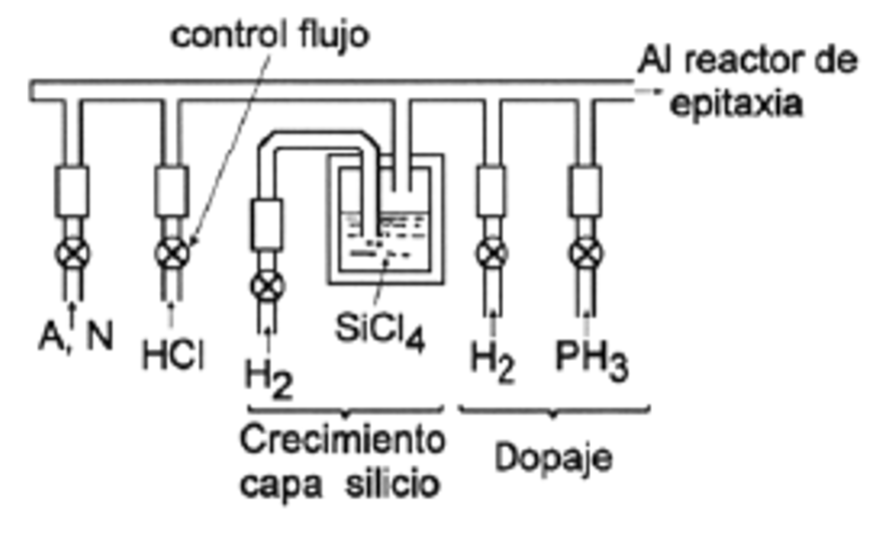
\includegraphics[width=0.5\linewidth]{Imagenes/Semiconductores - VPE.png}
    \caption{Epitaxia en fase vapor(VPE)}
\end{figure}

\begin{enumerate}
    \item Limpieza del aire del reactor con H2.
    \item Calentamiento del reactor.
    \item Ataque mediante HCl, a unos 1200ºC.
    \item Se introducen los gases con Si y dopantes para iniciar el crecimiento epitaxial.
    \item Se procede a inyectar N para eliminar restos de H2
\end{enumerate}

\section{Procesos de oxidación}
Consiste en la aportación de una capa protectora y aislante. Se utiliza para pasivar la superficie final de la oblea. Actúa como escudo protector contra agentes contaminantes externos. Proporciona aislamiento eléctrico. Las capas de SiO2 permiten obtener máscaras selectivas con tra la difusión de átomos dopantes.

\section{Proceso fotolitográfico}
Es un método de transferencia a la oblea de una imagen o cliché. 

\begin{enumerate}
    \item La imagen a procesar se pasa a una capa de resina depositada sobre el substrato.
    \item Se procede a la insolación por radiación ultravioleta que produce la polimerización de la resina no expuesta (negativa o positiva).
    \item La resina no polimerizada se elimina mediante lavado.
    \item La resina polimerizada que haya quedado actúa de escudo protector para las operaciones posteriores (ataque químico, deposición, dopado, etc.)
\end{enumerate}

\section{Deposición de dieléctricos y polisilicio}

Permite elaborar capas conductoras, de aislamiento eléctrico entre capas metálicas y de protección frente a ataques ambientales. Como requisitos debe cumplir que el espesor sea uniforme sobre toda la oblea, la estructura y composición debe ser reproducible y fácilmente controlable, y el proceso debe ser reproducible, automatizable y barato. Los materiales utilizados son: Silicio policristalino, Dióxido de Silicio y Nitruro de Silicio.

\section{Dopado}

Consiste en la formación de terminales de base y emisor (TTL) ó de fuente y drenador (MOS). Para ello la distribución de los dopantes ha de ser controlada en perfil y concentración. Este proceso se lleva a cabo por difusión ó por implantación iónica.

Tipos de difusión:
\begin{itemize}
    \item Sustitucional: El átomo dopante ocupa un hueco cedido por un átomo saliente de la estructura cristalina.
    \item Intersticial: El átomo dopante se encaja en el seno de la estructura, pero fuera de la red cristalina (requiere menor cantidad de energía).
    \item Intersticial modificado: Proceso mixto entre sustitucional é intersticial.
\end{itemize}

\section{Metalización de terminales}

Consiste en la deposición de las capas conductoras necesarias para la interconexión de dispositivos entre sí y con el exterior. Se pueden obtener con capas de polisilicio, o con aluminio.

Características:
\begin{itemize}
    \item Contacto de baja resistencia
    \item metal de alta conductividad
    \item Buena adherencia
    \item Definición fácil del patrón
    \item Fácil de atacar
    \item Compatibilidad con el resto de procesos
    \item Uniformidad en la deposición
    \item Resistente a corrosión
    \item Fácil conexionado por la electromigración
    \item No debe reaccionar con el semiconductor
\end{itemize}